\documentclass[12pt]{article}
\usepackage{listings}
\usepackage[colorlinks=true,pagebackref,linkcolor=blue]{hyperref}
\textwidth=7in
\textheight=9.5in
\topmargin=-1in
\headheight=0in
\headsep=.5in
\hoffset  -.85in

\lstset{
basicstyle=\footnotesize\ttfamily,
language=bash,
upquote=true,
breakatwhitespace=true,
columns=fullflexible,
keepspaces,
%numbers=none,
tabsize=3,
frame=blrt,
framextopmargin=5pt,
showstringspaces=false,
extendedchars=true
}

\pagestyle{empty}

\renewcommand{\thefootnote}{\fnsymbol{footnote}}

\begin{document}



\begin{center}
{\bf AMS 550.400 \quad HW SET 1\quad  Due Date:  Oct 8}\\
\vskip.2in
{\footnotesize Last Compiled on \today}
\end{center}

\setlength{\unitlength}{1in}

\begin{picture}(6,.1) 
\put(0,0) {\line(1,0){6.25}}         
\end{picture}

 

\renewcommand{\arraystretch}{2}

\vskip.25in
\noindent\textbf{Problem 1 (10 pts):}  
Assume that you are starting from ``scratch'' at the directory \verb+~/+.
Provide a sequence of git/bash commands that yields a git folder with 
a commit history such that:
\begin{itemize}
\item the \emph{master} branch has commits $A$, $B$, $C$, $X$ and $D$,
\item the \emph{alt} branch has commits $A$, $B$, $X$,
\end{itemize}
Suppose that you are currently working on \texttt{master} branch. Draw 
its commit history graph (i.e., the graph portion of the output of
\verb+git log --graph --oneline+).  Next, assume that 
you are on \texttt{alt} branch. Draw its commit history graph.  

\begin{enumerate}
\item mkdir hw1p1.git 
\item cd hw1p1.git 
\item git init . 
\item vi main.txt
\item git add .
\item git commit -m "A added to master"
\item vi main.txt
\item git add .
\item git commit -m "B added to master branch"
\item git branch alt
\item git branch
\item vi main.txt
\item git add .
\item git commit -m "C added to master branch"
\item git checkout alt
\item vi main.txt
\item git add .
\item git commit -m "X added to alt branch"
\item git checkout master
\item git merge alt
\item vi main.txt
\item git add .
\item git commit -m "Alt merged to master branch"
\item git branch
\item vi main.txt
\item git add .
\item git commit -m "D added to master branch"
\item git log --graph --oneline
\item git checkout alt
\item git log --graph --oneline
\end{enumerate}

\begin{figure}[h]
    \begin{center}
        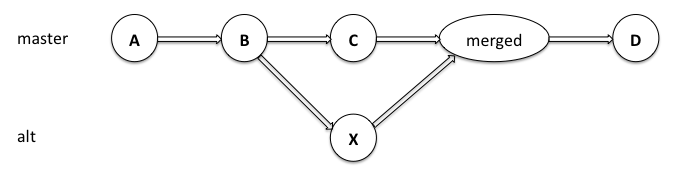
\includegraphics[width=\textwidth]{master_commitgraph.png}
    \end{center}
    \caption{WMATA existing lines and stations, June 2012}
    \label{fig:wmatamap}
\end{figure}

\begin{figure}[h]
    \begin{center}
        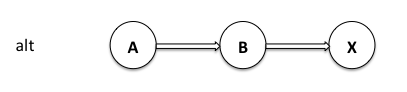
\includegraphics[width=\textwidth]{alt_commitgraph.png}
    \end{center}
    \caption{WMATA existing lines and stations, June 2012}
    \label{fig:wmatamap}
\end{figure}

\vskip.25in
\noindent\textbf{Problem 2 (10 pts):}
Assume that you are starting from ``scratch'' at the directory \verb+~/+.
Provide a sequence of git/bash commands that yields a git folder and 
\begin{itemize}
\item configure your git with your name and your email address,
\item set up an alias for each of the git remotes listed below:
\begin{verbatim}
git://github.com/nhlee/550400.stanza1.git 
git://github.com/nhlee/550400.stanza2.git 
git://github.com/nhlee/550400.stanza3.git 
\end{verbatim}
Assume that each remote contains exactly single commit with 
a txt file for a single (different) stanza,
\item pull to combine three stanzas of a poem,
\item after the first pull, add the title of the poem,
\item after the second and third pull, resolve the merge conflict,
\item after resolving the third pull merge conflict, push the result
  to your (newly created) remote repository. 
\end{itemize}

\begin{enumerate}
\item mkdir hw1p2.git
\item cd hw1p2.git
\item git init .
\item git remote add s1 git://github.com/nhlee/550400.stanza1.git
\item git pull s1 master
\item vi main.txt
\item git add .
\item git commit -m "Title added"
\item git remote add s2 git://github.com/nhlee/550400.stanza2.git
\item git pull s2 master
\item vi main.txt
\item git add .
\item git commit -m "2nd stanza merged"
\item git remote add s3 git://github.com/nhlee/550400.stanza3.git
\item git pull s3 master
\item vi main.txt
\item git add .
\item git commit -m "3rd stanza merged"
\item git remote add origin https://github.com/tangdnn/550400.homeworkset.1.git
\item git push origin master
\item git remote rm origin
\end{enumerate}


\newpage
\noindent\textbf{Problem 3 (40 pts):}
Consider a team of four students, say, $A$, $B$, $C$ and $D$, 
who just started working 
on writing a \texttt{latex/beamer} file, say \texttt{main.tex}, 
for a class presentation of their work statement.  
Assume that they do not wish to coordinate their schedules for a
concurrent group meeting (both virtually and physically).  
Assume that:
\begin{itemize}
\item $A$ is in charge of \emph{Introduction},
\item $B$ is of \emph{Problem Statement}, 
\item $C$ is of  \emph{Timeline},
\item $D$ is of \emph{Deliverable} part of the presentation.  
\end{itemize}
In other words, their contributions to \texttt{main.tex} do not overlap.
Then, 
\begin{itemize}
\item first, devise a work flow strategy for the team so that they can
  collaborate asynchronously using \texttt{git},
\item next, devise yet another \texttt{git} strategy different from your earlier
  proposal.  
\end{itemize}
Finally,
\begin{itemize}
\item discuss the strength and weakness of each of your proposed strategies in terms of merge
conflicts resolution,
\item make the final recommendation.  
\end{itemize}
In order to answer this question, \emph{build}
a mathematical model, \emph{following} the guideline from IMM. 
Use Section 1.4 and Section 1.5 of IMM as \emph{role models}.    
For example, you are to identify which variables  are exogenous 
and which are endogenous.  More specifically, among other things, 
in your model, is the preamble part of \texttt{main.tex} an endogenous 
or exogenous variable?  
Note also that in addition to this issue, there are other issues that
you are to consider.  So, \emph{be sure to consult IMM}. 

\vskip0.25in
\noindent\textbf{Problem 4 (aka.\ Fair Play, 40 pts):}
Answer the following question:
\begin{verse}
Is the tennis game fair?
\end{verse}
Note that unlike Problem 3, this question is vaguely stated.
This is intensional, whence to begin, you will first need to clarify
what exactly your question is.
You may use the class discussion on this particular 
problem, but you \emph{may not} directly refer to our 
discussion.  Instead, formulate the model carefully but concisely in 
your own words.   

\vskip0.25in
\noindent\textbf{Final Remarks about Problem 3 \& Problem 4:} 
They are open-ended problems.  However, your scores will be determined
by how well do you follow the exposition style outlined by IMM and
WMA.  For both problems, your write-up should be 
\begin{itemize}
\item self-contained,
\item covering all four parts of Section 1.3 of IMM,
\item paying a particular attention to any causal relation that you
  might be investigating, following Chapter 3 of WMA,
\item answering questions that are explicitly asked in the problem statements.
\end{itemize}
For Problem 3, focus mostly on Step 2 and Step 3 of Section
1.3 of IMM.  For Problem 4, focus mostly on Step 1 and Step
2.  For each problem, minimum 1 pages and maximum 2 pages.
\end{document}
